\subsubsection{Varying $c_L, a_R, b_R,$ and $c_R$ and fixing $a_L = b_L = 1$}

Now we will attempt to imitate the effects of the parameter $E_0$ on the branches $f_\B$ and $f_\D$ better.
Previously, we just varied $c_R$ which changes the values of the whole branches evenly.
Now, we only want to affect the value at the left borders of these branches.
For this, we introduce new parameters that are tied directly to characteristics of the model function.
To make this process easier, we scaled the model to the domain $[0, 4]$.
The adjusted model is $x_{n+1} = f(x_n) \mod 4$ with $f$ being defined by the following set of equations.
It is similar to the previous definition with the constant values adjusted.

\begin{align}
	f(x) & = \begin{cases}
		         g(x)     & \text{if } r(x) < 2 \\
		         g(x) + 2 & \text{else}
	         \end{cases}                                             \\
	g(x) & = \begin{cases}
		         g_L(x) = a_L \cdot s_L(x)^2 + b_L \cdot s_L(x) + c_L & \text{if } s(x) < 1 \\
		         g_R(x) = a_R \cdot s_R(x)^2 + b_R \cdot s_R(x) + c_R & \text{else}
	         \end{cases}
\end{align}
\begin{subequations}
	\begin{align}
		s(x)   & = x \mod 2           \\
		s_L(x) & = s(x) - \frac{1}{2} \\
		s_R(x) & = s(x) - \frac{3}{2}
	\end{align}
\end{subequations}

The new parameters are $g_R(1)$ for the value at the left border of branches $f_\B$ and $f_\D$, $g_R(2)$ for the value at the right border of the branches, and finally $\frac{d}{dx} g_R(x) |_{x = 2}$ for the slope of the branches at the right border.
We fix the parameter $\frac{d}{dx} g_R(x) |_{x = 2} = 1$ to have the maximum slope being $1$.
We also fix the parameter $g_R(2) = 2 + \epsilon$ with $\epsilon = 0.1$ to have the value at the right border of the branches just above the bisector $y = x$.
The parameter left is $g_R(1)$, the value at the left border of the branches.
This parameter is varied.

\todo{Solve for parameters $a_R, b_R, c_R$}

The cobwebs show that along these regions of the same period, the symbolic sequence evolves just like the symbolic sequence evolved in the original model along the chains of the same period.
Points of the sequence jump from branches $\A$ and $\C$ to branches $\B$ and $\D$.

\todo{changing the parameters of left branch gives us gecko formation}
Lighter areas indicate the existence of ``type B'' regions.

\todo{right branch has no local minimum and steepness relatively even => replace w linear branch}

Scaling the model to the interval $[0, 1]$ and mirroring the influence of the parameter $p_x$ will give the minimal model producing the desired bifurcation structures.

\todo{how scaled}

\begin{figure}
	\centering
	\includegraphics[width=0.6\textwidth]{40_Quadratic_fittingR/2D_Period_Whole/result.png}
	\caption{2D Scan of Periods of First Fitted Quadratic Model}
	\label{fig:quadratic.full.fit.1.Period}
\end{figure}

\begin{figure}
	\centering
	\begin{subfigure}{0.3\textwidth}
		\centering
		\includegraphics[width=\textwidth]{40_Quadratic_fittingR/Cobweb_A/result.png}
		\caption{At Point A}
		\label{fig:quad.full.fit.1.CobwebA}
	\end{subfigure}
	\begin{subfigure}{0.3\textwidth}
		\centering
		\includegraphics[width=\textwidth]{40_Quadratic_fittingR/Cobweb_B/result.png}
		\caption{At Point B}
		\label{fig:quad.full.fit.1.CobwebB}
	\end{subfigure}
	\begin{subfigure}{0.3\textwidth}
		\centering
		\includegraphics[width=\textwidth]{40_Quadratic_fittingR/Cobweb_C/result.png}
		\caption{At Point C}
		\label{fig:quad.full.fit.1.CobwebC}
	\end{subfigure}
	\caption{Cobwebs at Different Points}
	\label{fig:quad.full.fit.1.Cobwebs}
\end{figure}

\begin{figure}
	\centering
	\begin{subfigure}{0.4\textwidth}
		\centering
		\includegraphics[width=\textwidth]{41_Quadratic_fittingR_Gecko/2D_Period_Whole/result.png}
		\caption{Full Model}
		\label{fig:quadratic.full.fit.2.period.full}
	\end{subfigure}
	\begin{subfigure}{0.4\textwidth}
		\centering
		\includegraphics[width=\textwidth]{41_Quadratic_fittingR_Gecko/2D_Period_Whole/result-halved.png}
		\caption{Halved Model}
		\label{fig:quadratic.full.fit.2.period.halved}
	\end{subfigure}
	\caption{2D Scans of Periods of Adjusted Model...}
\end{figure}

\begin{figure}
	\centering
	\begin{subfigure}{0.3\textwidth}
		\centering
		\includegraphics[width=\textwidth]{41_Quadratic_fittingR_Gecko/Cobweb_A/result.png}
		\caption{At Point A}
		\label{fig:quad.full.fit.2.CobwebA}
	\end{subfigure}
	\begin{subfigure}{0.3\textwidth}
		\centering
		\includegraphics[width=\textwidth]{41_Quadratic_fittingR_Gecko/Cobweb_B/result.png}
		\caption{At Point B}
		\label{fig:quad.full.fit.2.CobwebB}
	\end{subfigure}
	\begin{subfigure}{0.3\textwidth}
		\centering
		\includegraphics[width=\textwidth]{41_Quadratic_fittingR_Gecko/Cobweb_C/result.png}
		\caption{At Point C}
		\label{fig:quad.full.fit.2.CobwebC}
	\end{subfigure}
	\caption{Cobwebs at Different Points}
	\label{fig:quad.full.fit.2.Cobwebs}
\end{figure}

\begin{figure}
	\centering
	\begin{subfigure}{0.4\textwidth}
		\centering
		\includegraphics[width=\textwidth]{50_Quadratic_linearR/2D_Period_Whole/result.png}
		\caption{Full Model}
		\label{fig:quadratic.full.fit.lin.period.full}
	\end{subfigure}
	\begin{subfigure}{0.4\textwidth}
		\centering
		\includegraphics[width=\textwidth]{50_Quadratic_linearR/2D_Period_Whole/result-halved.png}
		\caption{Halved Model}
		\label{fig:quadratic.full.fit.lin.period.halved}
	\end{subfigure}
	\caption{2D Scans of Periods of Adjusted Model...}
\end{figure}

\begin{figure}
	\centering
	\begin{subfigure}{0.3\textwidth}
		\centering
		\includegraphics[width=\textwidth]{50_Quadratic_linearR/Cobweb_A/result.png}
		\caption{At Point A}
		\label{fig:quad.full.fit.lin.CobwebA}
	\end{subfigure}
	\begin{subfigure}{0.3\textwidth}
		\centering
		\includegraphics[width=\textwidth]{50_Quadratic_linearR/Cobweb_B/result.png}
		\caption{At Point B}
		\label{fig:quad.full.fit.lin.CobwebB}
	\end{subfigure}
	\begin{subfigure}{0.3\textwidth}
		\centering
		\includegraphics[width=\textwidth]{50_Quadratic_linearR/Cobweb_C/result.png}
		\caption{At Point C}
		\label{fig:quad.full.fit.lin.CobwebC}
	\end{subfigure}
	\caption{Cobwebs at Different Points}
	\label{fig:quad.full.fit.lin.Cobwebs}
\end{figure}

\begin{figure}
	\centering
	\begin{subfigure}{0.4\textwidth}
		\centering
		\includegraphics[width=\textwidth]{99_Yunus/2D_Period_Zoomed/result.png}
		\caption{Original Model Full}
		\label{fig:quad.final.comparison.og.full}
	\end{subfigure}
	\begin{subfigure}{0.4\textwidth}
		\centering
		\includegraphics[width=\textwidth]{52_Quadratic_linearR_scaled_mirrored/2D_Period_Whole/result.png}
		\caption{Final Model Full}
		\label{fig:quad.final.comparison.fin.full}
	\end{subfigure} \\
	\begin{subfigure}{0.4\textwidth}
		\centering
		\includegraphics[width=\textwidth]{98_Yunus_modpi/2D_Period_Zoomed/result.png}
		\caption{Original Model Halved}
		\label{fig:quad.final.comparison.og.halved}
	\end{subfigure}
	\begin{subfigure}{0.4\textwidth}
		\centering
		\includegraphics[width=\textwidth]{52_Quadratic_linearR_scaled_mirrored/2D_Period_Whole/result-halved.png}
		\caption{Final Model Halved}
		\label{fig:quad.final.comparison.fin.halved}
	\end{subfigure}
	\caption{Comparison of 2D Scans of Periods of Original and Final Model}
	\label{fig:quad.final.comparison}
\end{figure}
